\documentclass[25pt,landscape]{foils}
%\usepackage{amsfonts}
%\usepackage{amsthm}
\usepackage[pdftex]{color}
\usepackage[pdftex]{graphicx}
\usepackage[pdftex]{geometry}
\geometry{headsep=2ex,hscale=0.9}
\pdfpagewidth=11in
\pdfpageheight=8.5in

\setlength{\footskip}{0.0in}
\setlength{\textheight}{9.0in}
\setlength{\topmargin}{.0in}

% Need to find the correct path to the file pdfcolor.tex on the next
% line!!!
\input /usr/share/texmf/pdftex/plain/misc/pdfcolor
%
% These files are used with PPower to create PowerPoint-like presentations
\usepackage{pause}
\usepackage{background}
\usepackage{pp4slide}
%\usepackage{pp4slide_BW}
%\usepackage{pdfscreen}

\newtheorem{Prop}{Proposition}
\newtheorem{Theo}{Theorem}

\newcommand{\br}{{\mathbf r}}
\newcommand{\bA}{{\mathbf A}}
\newcommand{\ba}{{\bf a}}
\newcommand{\bb}{{\bf b}}
\newcommand{\bc}{{\bf c}}
\newcommand{\bC}{{\bf C}}
\newcommand{\bd}{{\bf d}}
\newcommand{\bq}{{\bf q}}
\newcommand{\be}{{\bf e}}
\newcommand{\bh}{{\bf h}}
\newcommand{\bbm}{{\bf m}}
\newcommand{\bt}{{\bf t}}
\newcommand{\bs}{{\bf s}}
\newcommand{\bn}{{\bf n}}
\newcommand{\bu}{{\bf u}}
\newcommand{\bv}{{\bf v}}
\newcommand{\bw}{{\bf w}}
\newcommand{\bx}{{\bf x}}
\newcommand{\by}{{\bf y}}
\newcommand{\bbf}{{\bf f}}
\newcommand{\bH}{{\bf H}}
\newcommand{\bL}{{\bf L}}
\newcommand{\bM}{{\bf M}}
\newcommand{\bN}{{\bf N}}
\newcommand{\bS}{{\bf S}}
\newcommand{\bT}{{\bf T}}
\newcommand{\bD}{{\bf D}}
\newcommand{\bX}{{\bf X}}
\newcommand{\bY}{{\bf Y}}
\newcommand{\bP}{{\bf P}}
\newcommand{\bQ}{{\bf Q}}
\newcommand{\bI}{{\bf I}}
\newcommand{\bR}{{\bf R}}
\newcommand{\bU}{{\bf U}}
\newcommand{\bV}{{\bf V}}
\newcommand{\bW}{{\bf W}}
\newcommand{\bJ}{{\bf J}}
\newcommand{\bB}{{\bf B}}
\newcommand{\bzero}{{\bf 0}}
\newcommand{\bgamma}{{\mbox {\boldmath $\gamma$}}}
\newcommand{\btheta}{{\mbox {\boldmath $\theta$}}}
\newcommand{\bLambda}{{\mbox {\boldmath $\Lambda$}}}
\newcommand{\bPsi}{{\mbox {\boldmath $\Psi$}}}
\newcommand{\bPhi}{{\mbox {\boldmath $\Phi$}}}
\newcommand{\bcS}{{\mbox {\boldmath ${\cal S}$}}}
\newcommand{\bcH}{{\mbox {\boldmath ${\cal H}$}}}
\newcommand{\bcI}{{\mbox {\boldmath ${\cal I}$}}}
\newcommand{\bcR}{{\mbox {\boldmath ${\cal R}$}}}
\newcommand{\bcB}{{\mbox {\boldmath ${\cal B}$}}}

\zerolistvertdimens

\begin{document}
\raggedright

\color{white}
%\color{black}
\pagecolor{bgcolor} % set background color
\definecolor{bgblue}{rgb}{0.04,0.37,0.59}
\definecolor{wh2}{rgb}{0.35,0.74,0.98}
%\vpagecolor{bgblue}
\pagecolor{bgblue}

\definecolor{htext}{rgb}{0.98,0.98,0.04}


\foilhead{\LARGE On Interference Cancellation for Synchronous CDMA}
\begin{center}
\vspace{0.8in}
{\large \bf Shu Wang, James Caffery, Jr., and Hanhong Shen} \vspace{1em} \\
{\it University of Cincinnati \\ Dept. of Electrical \& Computer
Engineering \\ \& Computer Science \\ Cincinnati,
OH~~45221-0030 \vspace{2em} \\
{\bf ISWC 2002 \\ Victoria, BC, Canada}}
\end{center}

\foilhead[-.4in]{Introduction}
\begin{itemize}
\item CDMA techniques have attracted attention for their
spectral efficiency, interference resistance and flexible traffic
control.
\item MAI is the dominant impairment for CDMA systems and exits even with
perfect power control.
%\item Multiuser detection describes method that minimize the effects of
%MAI and mitigate the near-far problem.
%\item Interference cancellation provides a promising alternative
%to the conventional or optimum detectors in multiuser detection.
\item Multiuser detection promising approach to mitigate MAI:
multiuser detectors (linear/nonlinear) and interference cancellation
\item We explore interference cancellation in a framework that leads to an
interference cancellation representation of linear multiuser detectors (DD,
MMSE, MAME)
 \begin{itemize}
 \item Direct interference cancellation (D-IC)
 \item MMSE interference cancellation (MMSE-IC)
 \item MAME interference cancellation (MAME-IC)
 \end{itemize}
\end{itemize}

\foilhead[-.5in]{Data Model}
\begin{itemize}
\zerolistvertdimens
\item Consider a synchronous CDMA system with $L$ chips
per bit ($T_{b}=L T_{c}$).
\item Received signal, after chip-matched filter followed by chip-rate
sampling: \vspace{-.2in}
$$
\br = \sum_{k=1}^{K} A_{k} b_{k} \bs_{k} + \bn \; = \; \bS \bA \bb  + \bn
$$
where $\bA={\sf diag}\left\{ A_{1} \; A_{2} \; \ldots \; A_{K} \right\}$,
$\bS=\left[ \bs_{1} \; \bs_{2} \; \ldots \; \bs_{K} \right]$ and $\bb =
\left[ b_{1} \; b_{2} \; \ldots \; b_{K} \right]^{T}$ with $b_{i} \in
\left\{ +1,-1 \right\}$.
\item Linear multiuser detectors can be written in the form  \vspace{-.2in}
$$
\bb = {\sf sgn} \left\{ \bW \br \right\} \vspace{-.2in}
$$
or for the $k$th user {\color{htext} $b_{k} = {\sf sgn} \left\{ \bw^{T}_{k}
\br \right\}$} where $\bw_{k}^{T}$ is the $k$th row of $\bW$.
\item We consider detection of user 1's data only.
\item Maintain the restriction that $L>K$.
\end{itemize}

\foilhead[-.5in]{Data Model w.r.t. User 1}
\begin{itemize}
\item In terms of user 1: \vspace{-.2in}
\begin{eqnarray*}
\br & = & A_{1}b_{1}\bs_{1} + \sum_{k=2}^{K} A_{k} b_{k} \bs_{k} + \bn \\
 & = & \left[ \matrix{\bs_{1} & \tilde{\bS}} \right] \left[ \matrix{ A_{1}
 & \bzero^{T} \cr \bzero & \tilde{\bA} } \right] \left[ \matrix{ b_{1} \cr
 \tilde{\bb}} \right] + \bn \\
 & = & A_{1}b_{1} \bs_{1} + \tilde{\bS} \tilde{\bA} \tilde{\bb} +\bn \\
 & = & A_{1}b_{1} \bs_{1} + \bbm_{1} + \bn
\end{eqnarray*}
where $\bbm_{1} = \tilde{\bS}\tilde{\bA}\tilde{\bb}$ is the MAI seen by
user 1, and
\begin{eqnarray*}
\tilde{\bS} & = & \left[ \bs_{2} \; \bs_{3} \; \ldots \; \bs_{K} \right] \\
\tilde{\bA} & = & {\sf diag} \left\{ A_{2} \; A_{3} \; \ldots \; A_{K}
\right\} \\
\tilde{\bb} & = & \left[ b_{2} \; b_{3} \; \ldots \; b_{K} \right]^{T}
\end{eqnarray*}
\end{itemize}

\foilhead[-.5in]{Interference Cancellation (IC)}
\begin{itemize}
\zerolistvertdimens
\item Goal: estimate $\bbm_{1}$ and remove from $\br$.
\centerline{\includegraphics[width=9in]{IC_block}}
\item Given an estimate of MAI, $\hat{\bbm}_{1}$, the estimate of user 1's
data bit is \vspace{-.2in}
\begin{eqnarray*}
\hat{b}_{1} & = & {\sf arg} \; \min_{b} \left\| \br - \hat{\bbm}_{1} -
A_{1}b \bs_{1} \right\| \\
 & = & {\sf sgn} \left\{ \bs_{1}^{T} \left( \br - \hat{\bbm}_{1} \right)
 \right\} \\
 & = & {\sf sgn} \left\{ A_{1}b_{1} + \bs_{1}^{T} \left( \bbm_{1} -
 \hat{\bbm}_{1} \right) + \bs_{1}^{T} \bn \right\}
\end{eqnarray*}
\item If we assume $\hat{\bbm}_{1} = \bW_{1} \br$, then  \vspace{-.2in}
$$
\hat{b}_{1} = {\sf sgn} \left\{ \bs_{1}^{T} \left( \bI_{L} - \bW_{1}
\right) \br \right\} = {\sf sgn} \left\{ \bs_{1}^{T} \bW^{IC}_{1} \br \right\}
 = {\sf sgn} \left\{ \left[\bw_{1}^{IC} \right]^{T} \br \right\}
 \vspace{-.2in}
$$
\item Therefore, can represent IC as a linear filter.
\end{itemize}

\foilhead[-.3in]{Types of IC}
\begin{itemize}
\zerolistvertdimens
% Interference cancellation typically requires less implementation
%complexity while offering similar performance compared to the
%linear/nonlinear (????) detectors.
\item  Parallel interference cancellation (PIC): All users are
simultaneously demodulated and detected in a parallel behavior
(Jacobi Iteration).
\item  Successive/Serial interference cancellation (SIC): A
decision for the strongest user is made first and the interference
from this user is subsequently removed for the detection of the next
stronger user's data, etc.  (Gauss-Siedel Iteration)
\item Hybrid parallel/serial cancellation
\item Groupwise interference cancellation
\item Categories:
 \begin{itemize}
 \item Hard --- make decision on other user's bits, re-form interfering
 signal and remove.
 \item Soft --- estimate each user's interference, $A_{k}b_{k}\bs_{k}$, and
 remove.
 \end{itemize}
\end{itemize}

\foilhead[-.6in]{Direct Interference Cancellation (D-IC)}
\begin{itemize}
\zerolistvertdimens
\item Estimate $\hat{\bbm}_{1}$ according to the least
squares (LS) criterion.
\item  Estimate MAI $\hat{\bbm}$ by solving \vspace{-.2in}
$$
\hat{\bbm}_{1}^{D-IC} = \mbox{arg} \min_{\bbm} \left\| \br-\bbm-A_1 b_{1}
\bs_1 \right\|_2  \vspace{-.2in}
$$
subject to $\bbm\in\mbox{span}\{\tilde{\bS}\}$.
\item Since ideally $\hat{\bbm}_{1} = \tilde{\bS} \tilde{\bA} \tilde{\bb} =
\tilde{\bS} \hat{\bx}_{1}$, we can formulate $\hat{\bbm}_{1}^{D-IC}$ by
finding \vspace{-.2in}
$$
\hat{\bx}_{1} = {\sf arg} \; \min_{\bx} \left\| \br - A_{1}b_{1}\bs_{1} -
\tilde{\bS} \bx \right\|_{2}
$$
\item To separate the MAI from the observation vector, we use a unitary
matrix $\bQ$ to perform the Householder transformation on $\bs_{1}$
such that \vspace{-.2in}
$$
\bQ^{T} \bs_{1} = \left[ \matrix{ c & \bzero^{T}} \right]^{T} \vspace{-.1in}
$$
where $c = \pm \|\bs_{1}\| = \pm 1$ and \vspace{-.6in}
$$
\bQ = \bI_{L}-2\bq\bq^{T} \mbox{\hspace{.25in} with \hspace{.2in}} \bq =
\kappa %\frac{1}{\sqrt{2c(c-1)}}
\left[ \matrix{ s_{11}-c \cr s_{12} \cr \vdots \cr
s_{1L} } \right]
$$
\end{itemize}

\foilhead[-.5in]{Final Form of $\hat{\bbm}_{1}^{D-IC}$}
\begin{itemize}
\zerolistvertdimens
\item Applying $\bQ$ to $\br$ results in
$$
\bQ^{T} \br = \left[ \matrix{ r_{1} \cr \br_{M}} \right] \hspace{.3in} \&
\hspace{.3in} \bQ^{T}\bS = \bQ^{T} \left[ \matrix{\bs_{1} & \tilde{\bS}}
\right] = \left[ \matrix{ c & \bs_{M1}^{T} \cr \bzero & \tilde{\bS}_{M}}
\right]
$$
\item Using the Householder transformation, we can write
\begin{eqnarray*}
\mbox{arg} \min_{\bx} \left\| \tilde{\bS}\bx - \left( \br -
A_{1}b_{1}\bs_{1} \right) \right\| & = & \mbox{arg} \min_{\bx} \left\| \bS
\left[ \matrix{ A_{1}b_{1} \cr \bx}\right] - \br \right\| \\
 & & \hspace{-2in} = \mbox{arg} \min_{\bx} \left\| \left[ \matrix{ c & \bs_{M1}^{T} \cr
 \bzero & \tilde{\bS}_{M} } \right] \left[ \matrix{ A_{1}b_{1} \cr \bx
 }\right] - \left[ \matrix{ r_{1} \cr \br_{M}}
 \right] \right\| \\
 & & \hspace{-2in} = \mbox{arg} \min_{\bx} \left\| \left[ \matrix{ A_{1}b_{1} \cr \bx}
 \right] - \left[ \matrix{ \frac{r_{1}}{c} - \frac{1}{c} \bs_{M1}^{T}
 \tilde{\bS}_{M} \br_{M} \cr \tilde{\bS}_{M}^{+} \br_{M} } \right] \right\|
\end{eqnarray*}
so that $\hat{\bx}_{1} = \tilde{\bS}_{M}^{+}\br_{M}$ which is an estimate
of $\tilde{\bA}\tilde{\bb}$.
\end{itemize}

\foilhead[-.5in]{Detection of $b_{1}$}
\begin{itemize}
\zerolistvertdimens
\item Thus, $\hat{\bbm}^{D-IC}_{1} = \tilde{\bS}\tilde{\bS}_{M}^{+}
\br_{M}$.
\item The decision for the data bit of user 1 is given by \vspace{-.2in}
\begin{eqnarray*}
\hat{b}_{1}^{D-IC} & = & {\rm sgn} \left\{ \bs_{1}^{T} \left( \br -
\hat{\bbm}_{1}^{D-IC} \right) \right\} \\
 & = & {\rm sgn} \left\{ \bs_{1}^{T} \left( \bI_{L} - \tilde{\bS}
 \tilde{\bS}_{M}^{+} \left[ \matrix{ \bzero & \bI_{L-1}} \right] \bQ^{T}
 \right) \br \right\}
\end{eqnarray*}
\item Can represent the decision for $b_{1}$ as the output of a linear
filter: $\hat{b}_{1} = \mbox{sgn} \left\{ \bw_{1}^{T} \br \right\}$ where \vspace{-.3in}
$$
\bw_{1} = \left( \bI_{L} - \bQ \left[ \matrix{ \bzero^{T} \cr \bI_{L-1}}
\right] \tilde{\bS}_{M}^{+T} \tilde{\bS}^{T} \right) \bs_{1}
$$
\end{itemize}
\centerline{\includegraphics[width=10in]{DIC_block}}

\foilhead[-.6in]{MMSE Interference Cancellation (MMSE-IC)}
\begin{itemize}
\zerolistvertdimens
\item Minimize the MSE at the output of the MF for user 1 (i.e., input to
the slicer)
\item The MMSE estimate of the MAI, $\hat{\bbm}_{1}^{MMSE-IC}$ is \vspace{-.2in}
$$
\hat{\bbm}_{1}^{MMSE-IC} = \mbox{arg} \min_{\bbm} \; \mbox{E} \left\{ \left[
\bs_{1}^{T} \left( \br - A_{1}b_{1}\bs_{1} - \bbm \right) \right]^{2}
\right\}
% & = & \mbox{arg} \min_{\bbm} \; \mbox{E} \left\{ \left[ \bs_{1}^{T}
% \left( \bbm - \hat{\bbm} \right) \right]^{2} \right\}
$$
\item Find MMSE result with (change of variables) \vspace{-.2in}
$$
\hat{\bbm}_{1}^{MMSE-IC} = \bs_{1} \bw_{1}^{T} \br \vspace{-.30in}
$$
where  \vspace{-.7in}
$$
\bw_{1} = \mbox{arg} \min_{\bw} \; \mbox{E} \left\{ \left[ \bs_{1}^{T} \left(
\br - A_{1}b_{1}\bs_{1} \right) - \bw^{T} \br \right]^{2} \right\}
\vspace{-.1in}
$$
\item The optimal $\bw_{1}$ is \vspace{-.25in}
$$
\bw_{1} = \left( \bS \bA^{2} \bS^{T} + \sigma^{2} \bI_{L} \right)^{-1} \left(
\tilde{\bS} \tilde{\bA}^{2} \tilde{\bS}^{T} + \sigma^{2} \bI_{L} \right)
\bs_{1} \vspace{-.25in}
$$
so that \vspace{-.25in}
$$
\hat{\bbm}_{1}^{MMSE-IC} = \left( \tilde{\bS} \tilde{\bA}^{2}
\tilde{\bS}^{T} + \sigma^{2} \bI_{L} \right) \left( \bS \bA^{2} \bS^{T} +
\sigma^{2} \bI_{L} \right)^{-1} \br
$$
\end{itemize}

\foilhead[-.6in]{MMSE-IC {\small (cont)}}
\begin{itemize}
\item The decision for user 1's data bit is \vspace{-.2in}
\begin{eqnarray*}
\hat{b}_{1} & = & \mbox{sgn} \left\{ \bs_{1}^{T} \left( \br -
\hat{\bbm}_{1}^{MMSE-IC} \right) \right\} \\
 & = & \mbox{sgn} \left\{ \bs_{1}^{T} \left[ \bI_{L} - \left( \tilde{\bS}
 \tilde{\bA}^{2} \tilde{\bS}^{T} + \sigma^{2} \bI_{L} \right) \left( \bS
 \bA^{2} \bS^{T} + \sigma^{2} \bI_{L} \right)^{-1} \right] \br \right\}
\end{eqnarray*} \vspace{-.4in} \\
and the linear filter representation is \vspace{-.2in}
$$
\bw_{1}^{MMSE-IC} = \left[ \bI_{L} - \left( \bS \bA^{2} \bS^{T} +
\sigma^{2} \bI_{L}\right)^{-1} \left( \tilde{\bS} \tilde{\bA}^{2}
\tilde{\bS}^{T} + \sigma^{2} \bI_{L} \right) \right] \bs_{1}
$$
\end{itemize}
\centerline{\includegraphics[width=10in]{MMSEIC_block}}

\foilhead[-.5in]{Maximum Asymptotic Multiuser Efficiency IC (MAME-IC)}
\begin{itemize}
\zerolistvertdimens
\item Let $\hat{\bbm}_{1}^{MAME-IC} = \bs_{1} \bw_{1}^{T} \br$ \enspace .
\item The error probability for user 1 is
$$
P_{e1} = \mbox{E} \left[ Q\left( \frac{A_1b_1+ \sum_{k=2}^{K} A_kb_k\rho_{1k}
-\sum_{k=1}^K A_kb_k \bw_{1}^{T} \bs_k}
{\sigma \|\bs_1-\bw_{1}\|_2}\right)\right]
$$
\item The asymptotic multiuser efficiency (AME) of user 1 is
%given by the square of the smallest argument in $Q(\cdot)$ above normalized by $A_1^2/\sigma^2$:
$$
\eta_1(\bw_{1}) = {\max}^2 \left\{ 0\; ,\; \frac{1-\bs_1^T\bw_{1} -
\sum_{k=2}^{K} \frac{A_k}{A_1} \left| \rho_{1k}-\bs_k^T\bw_{1}\right|  }
{\|\bs_1-\bw_{1}\|_2} \right\}
$$
\item Choose $\bw_{1}$ to maximize the AME.
\end{itemize}

\foilhead[-.5in]{MAME-IC Solution}
\begin{itemize}
\zerolistvertdimens
\item Solving for $\bw_{1}$ does not permit a close-form solution for
$K>2$.
\item For $K=2$, the $\bw_{1}$ that maximizes AME is \vspace{-.2in}
\begin{eqnarray*}
\bw_{1} & = & \left\{ \begin{array}{ll}{A_1\over
A_2}\mbox{sgn}(\rho)\bs_2 ,&\mbox{if }{A_2\over A_1}<|\rho| ,\\
\rho\bs_2 ,&\mbox{otherwise.}\end{array}\right. \\
 & = & \mbox{sgn}(\rho) \max \left\{ |\rho|, \frac{A_{1}}{A_{2}} \right\}
 \bs_{2}
\end{eqnarray*} \vspace{-.4in} \\
\item Thus, the MAME estimate of the MAI is \vspace{-.2in}
$$
\hat{\bbm}_{1}^{MAME-IC} = \mbox{sgn}(\rho) \max \left\{ |\rho|,
\frac{A_{1}}{A_{2}} \right\} \bs_{1} \bs_{2}^{T} \br
$$
\centerline{\includegraphics[width=10in]{MAMEIC_block}}
\end{itemize}

\foilhead[-.7in]{Equivalence: D-IC and DD}
\begin{itemize}
\zerolistvertdimens
\item Consider the transformed received signal vector  \vspace{-.25in}
$$
\bQ^{T} \br = \left[ \matrix{ s_{11} & \bs_{M1}^{T} \cr \bzero &
\tilde{\bS}_{M} } \right] \bA \bb + \bQ^{T}\bn \vspace{-.25in}
$$
\item The decorrelating detector (DD) provides the minimum norm estimate of
$\bA\bb$ as \vspace{-.25in}
$$
\bA\bb = \left[ \matrix{ s_{11} & \bs_{M1}^{T} \cr \bzero & \tilde{\bS}_{M} }
\right]^{+} \bQ^{T}\br = \bS^{+} \bQ^{-T} \bQ^{T} \br = \bS^{+}\br \vspace{-.25in}
$$
\item The DD decision rule is  \vspace{-.25in}
$$
\hat{b}_{1}^{DD} = \mbox{sgn} \left\{ \left[ \matrix{ s_{11}^{-1} &
-s_{11}^{-1} \bs_{M1}^{T} \tilde{\bS}_{M}^{+} } \right] \bQ^{T} \br
\right\} \vspace{-.25in}
$$
\item The D-IC decision rule can be written as \vspace{-.25in}
\begin{eqnarray*}
\hat{b}_{1}^{D-IC} & = & {\rm sgn} \left\{ \bs_{1}^{T} \left( \bI_{L}
- \tilde{\bS} \tilde{\bS}_{M}^{+} \left[ \matrix{ \bzero & \bI_{L-1}}
\right] \bQ^{T} \right) \br \right\} \\
 & = & \mbox{sgn} \left\{ \left[ \matrix{ s_{11} &
-s_{11} \bs_{M1}^{T} \tilde{\bS}_{M}^{+} } \right] \bQ^{T} \br
\right\}
\end{eqnarray*} \vspace{-.6in} \\
\item Hence, $\bw_{1}^{D-IC} = s_{11}^{2} \bw_{1}^{DD}$.
\end{itemize}

\foilhead[-.5in]{Geometric Interpretation}
%\centerline{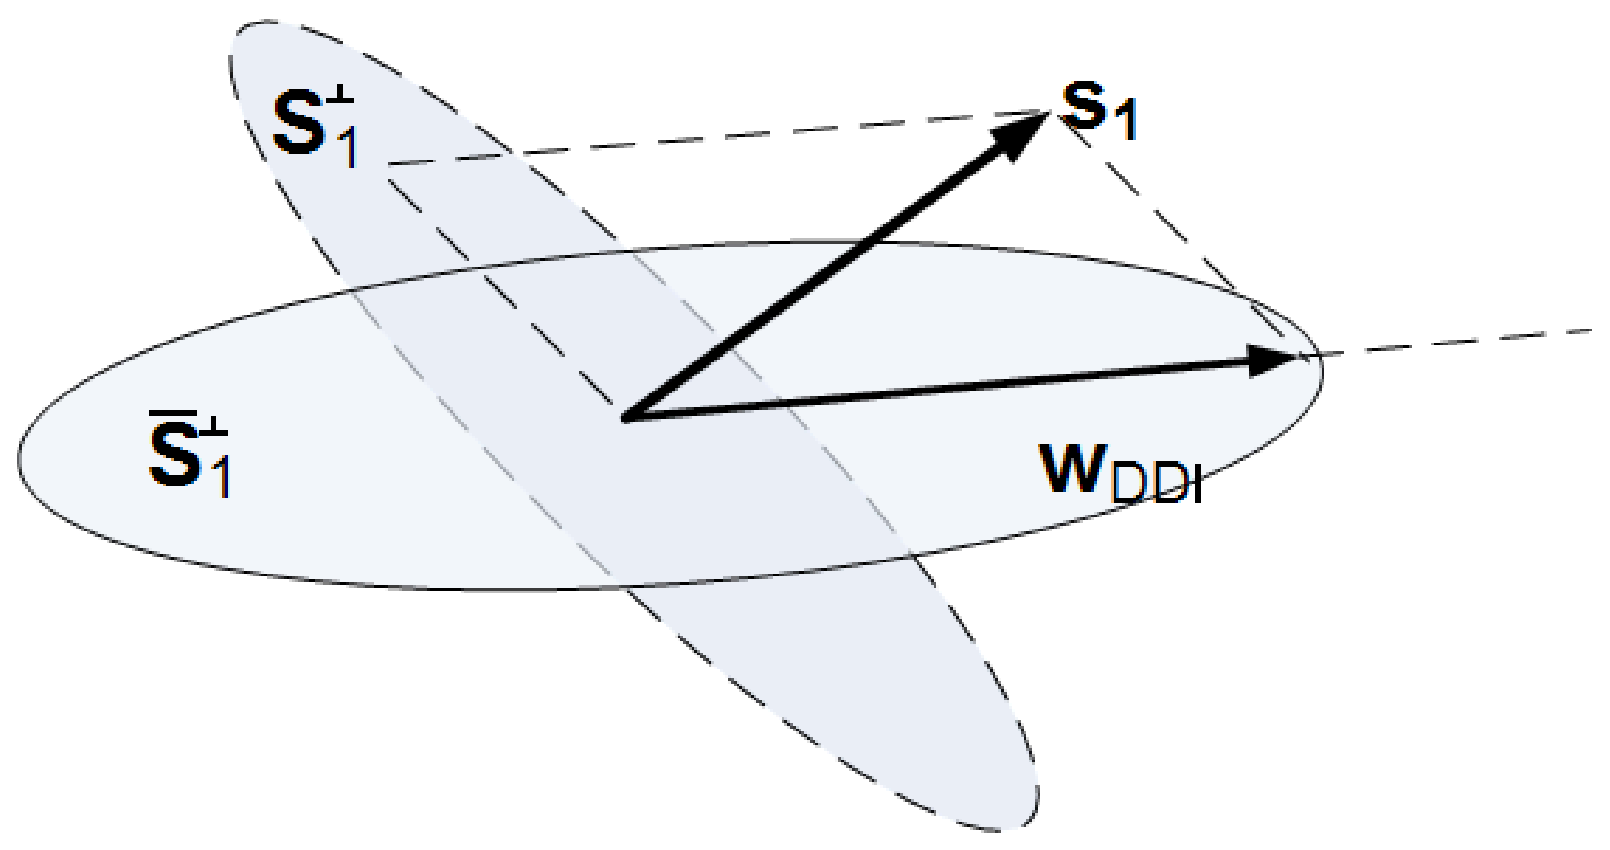
\includegraphics[width=5.50in]{DD_geometric}}
{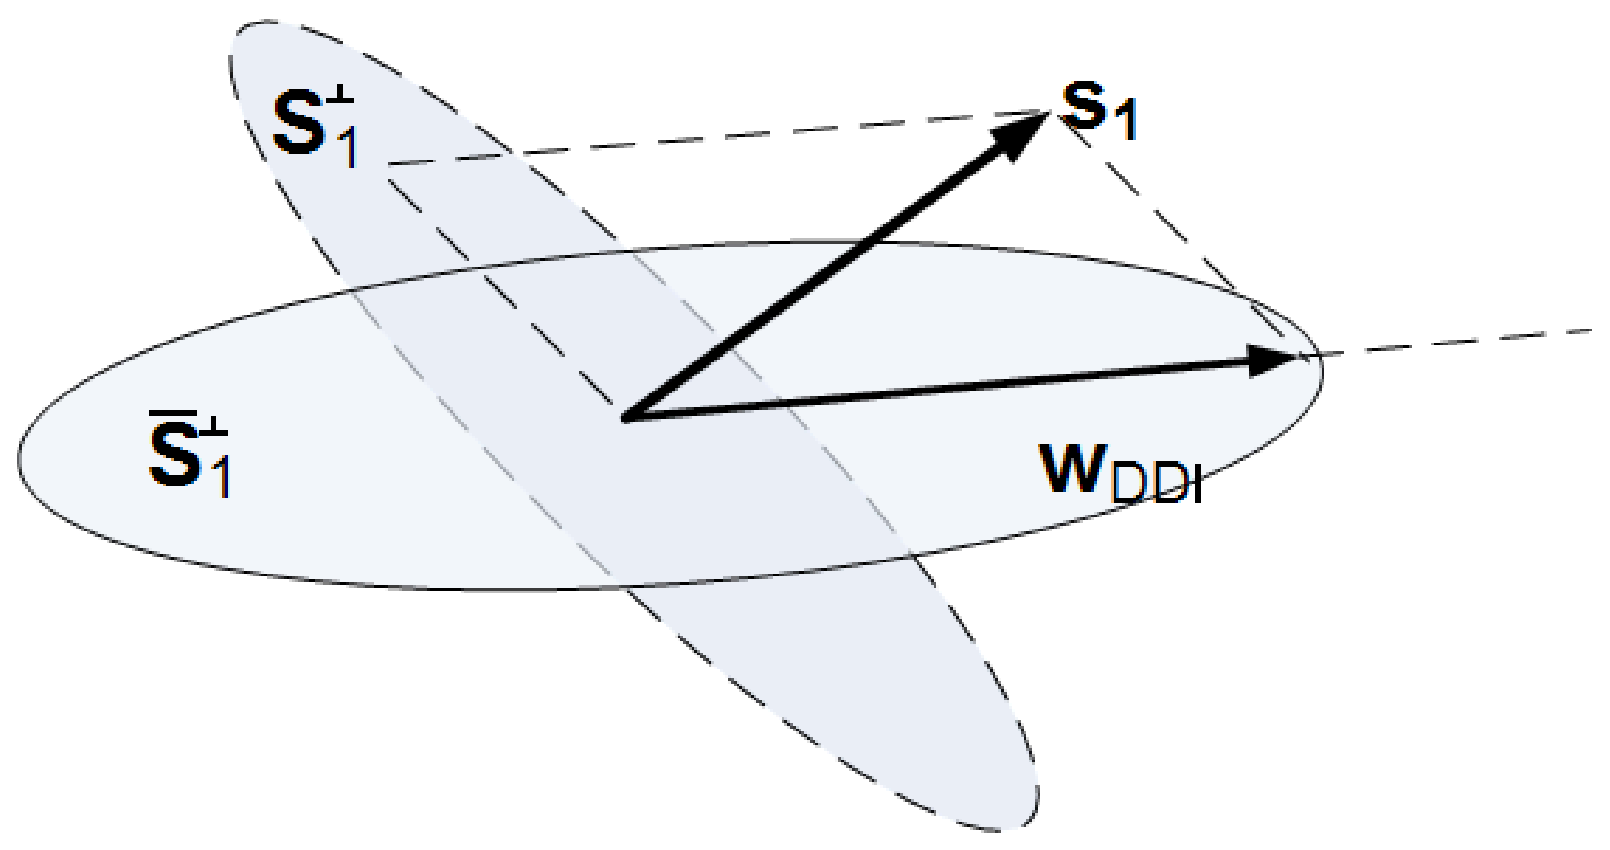
\includegraphics[width=5.50in]{DD_geometric}} \vspace{-.7in}\\
%\centerline{\includegraphics[width=5.0in]{DIC_geometric}}
\hfill{\includegraphics[width=5.0in]{DIC_geometric}}

\foilhead[-.6in]{Equivalences}
\begin{itemize}
\zerolistvertdimens
\item MMSE-IC and Linear MMSE
 \begin{itemize}
 \item Linear MMSE can be written as \vspace{-.2in}
 $$
 \bw_{1}^{MMSE} = \left( \bS \bA^{2} \bS^{T} + \sigma^{2} \bI_{L} \right)^{-1} \bs_{1} \vspace{-.2in}
 $$
 \item MMSE-IC can be simplified to \vspace{-.2in}
 $$
 \bw_{1}^{MMSE-IC} = A_{1}^{2} \left( \bS \bA^{2} \bS^{T} + \sigma^{2} \bI_{L} \right)^{-1} \bs_{1} \vspace{-.2in}
 $$
 %\item Thus, $\bw_{1}^{MMSE-IC} = A_{1}^{2} \bw_{1}^{MMSE}$ \enspace.
 \end{itemize}
\item MAME-IC and Linear MAME
 \begin{itemize}
 \item The decision variable for the MAME-IC can be written as \vspace{-.2in}
 $$
 \hat{b}_{1}^{MAME-IC} = \mbox{sgn} \left\{ \bs_{1}^{T} \br -
 \bw_{1}^{T} \br \right\} \vspace{-.2in}
 $$
 which results in the over linear filter operation  \vspace{-.2in}
 $$
 \bw_{1}^{MAME-IC} = \left\{ \begin{array}{ll} \bs_{1} -
 \frac{A_{1}}{A_{2}} \mbox{sgn}\{\rho\} \bs_{2} &  \mbox{ if }
 \frac{A_{2}}{A_{1}} < |\rho| \\ \bs_{1} - \rho \bs_{2}, & \mbox{
 otherwise} \end{array} \right. \vspace{-.2in}
 $$
 which is the same as the linear MAME.
 \end{itemize}
\end{itemize}


\foilhead{Conclusions}
\begin{itemize}
\item Considered a framework for interference cancellation in which MAI is
removed before MF detection of user 1.
\item Can be extended to other users.
\item Interference cancelers could be written as a linear filtering
operation.
\item Proposed IC's (D-IC, MMSE-IC and MAME-IC) were shown to be equivalent
to their linear multiuser detector counterparts (DD, MMSE, MAME).
\item IC's essentially a form of re-formulating the linear multiuser
detectors.
\end{itemize}

\end{document}
